% ------------------------------------
% INTRODUCTION
% ------------------------------------
\section{Introduction}
\label{sec:Introduction}
This section will describe the context of this theme, namely:
\begin{itemize}
  \item What is the scope of the theme?
  \item What is the actual state of the theme?
  \item What are the main difficults confronted?
\end{itemize}
% -------------------------------------
% INTERNET OF THINGS
% -------------------------------------
\subsection{Internet of Things}
\label{sub:Internet of Things}
The Internet of Things (IoT) is a concept in which the virtual world of information technology integrates seamlessly
with the real world of things \cite{Uckelmann:2011:AIT:2018904}. Through the amount of computer and network devices
available nowadays, the real world becomes accessible to business as well everyday scenarios. A more precise definition
of what is Internet of Things was formulated in the Strategic Research Agenda of the Cluster of European Research Projects
on the Internet of Things (CERP-IoT 2009):\\

``\textit{Internet of Things (IoT) is (...) a dynamic global network infrastructure with self configuring capabilities based on standard and interoperable
  communication protocols where physical and virtual `things' have identities, physical attributes, and virtual personalities and use intelligent interfaces,
  and are seamlessly integrated into the information network. In the IoT, `things' are expected to become active participants in business, information and social
  processes where they are enabled (...) by exchanging data and information  sensed about the environment, while reacting autonomously to the `real/physical world'
  events and influencing it by running processes that trigger actions and create services with or without direct human intervention. Interfaces in the form of services
  facilitate interactions with these `smart things' over the Internet (...) taking into account security and privacy issues.}''\\

IoT provides access to a more detailed information, which results that the level of analysis can be performed in a large-scale perspective, as well in a small-scale
perspective. But Internet of Things is more than a tool for managing business processes more efficiently and more effectively, IoT will also enable a more convenient life for all peoples.
Recently, IoT became relevant to industry and end-users\cite{Uckelmann:2011:AIT:2018904}, mainly because the reduction of cost and miniaturization of technologies used in IoT applications, such as RFID, sensor networks, NFC and
wireless communication. Technologies like these allows the detection of status of things, which toghether with collection and processing of detailed data,
allows to create an interactive and responsive network with huge potential for citizens, consumers, business and where is possible to gather immediate responses
to events that occurs in the real world\cite{Uckelmann:2011:AIT:2018904}. One of the expectations regarding of IoT concerns with real-world awareness provided to information systems \cite{mattern2010internet}.
An example is in logistics applications, by the use of RFID, companies can react promptly to relevant physical events, and then manage their processes in a better way,
typically increasing efficiency and reducing costs. Another expectation of IoT concerns with providing services to the end-users through common objects, in that
way products will be able to provide recommendations for use and maintenance instructions, supply warranty information or highlight complementary products.\\
% ---------------------------------------
% CLOUD COMPUTING
% ---------------------------------------
\subsection{Cloud Computing}
\label{sub:Cloud Computing}
This section will describe what is the concept of Cloud Computing? What is the most benefits of Cloud Computing?
How Internet of Things could take advantage of Cloud Computing?\\
% ---------------------------------------
% SMART SPACE
% ---------------------------------------
\subsection{Smart Space}
\label{sub:Smart Space}
In the context of this work, a smart space can be defined as an ecosystem composed by smart objects such as RFID tags and sensors, that are able to
acquire knowledge about this environment and also to adapt this inhabitants in order to improve their experience in that environment \cite{cook2004smart}.
In particular, the deployment of IoT applications in a smart space is a challenge today due the heterogenity of the smart objects that are present in a smart space
and also because the required infrastructure. In order to decrease the complexity of the deployment of an IoT application in a smart space, the Cloud computing paradigm allows to
virtualize the required physical infrastructure. Nowadays the infrastructure needed by IoT applications can be virtualized by Cloud providers such as Amazon Web Services
and Google Compute Engine, which helps to gain more flexibility and reduce the costs in the deployment of an IoT application. Therefore, another challenge concerns with the heterogenity
of a smart space, more precisely the variety of smart objects that can be inside of a given space. Many of these objects uses different communication protocols and drivers to communicate with devices,
the configuration of this objects must be manually handled, which makes the integration of these objects in the deployment of IoT applications in a smart space a inneficient process.  
% ----------------------------------------
% TOSCA
% ----------------------------------------
\subsection{TOSCA}
\label{sub:TOSCA}
This section will introduce the TOSCA standard and its main components.
% -----------------------------------------
% OPENTOSCA
% -----------------------------------------
\subsection{OpenTOSCA}
\label{sub:OpenTOSCA}
OpenTOSCA is an open-source framework developed by the University of Stuttgart that provides an ecosystem for the OASIS Topology and Orchestration Specification for
Cloud Applications (TOSCA) standard. OpenTOSCA allows to describe the components and relations of the applications, perform the orchestration and explicitly modeling
management aspects of the applications. The components of OpenTOSCA will be described with further detail at the following sections.
% ------------------------------------------
% OPENTOSCA CONTAINER
% ------------------------------------------
\subsubsection{OpenTOSCA Container}
\label{subs:OpenTOSCA Container}
OpenTOSCA Container is a runtime supporting imperative processing of TOSCA applications \cite{OpenTOSCA}. Imperative means that deployment and management services is realized through plans.
OpenTOSCA main tasks consists in management operations, run plans and manage state. At Fig\ref{fig:open_container} the architecture of OpenTOSCA Container is illustrated, as well
a processing sequence regarding the instantiation of a Cloud application.
% -------------------------------------------
% OPENTOSCA ARCHITECTURE
% -------------------------------------------
\begin{figure}[h!]
  \centering
  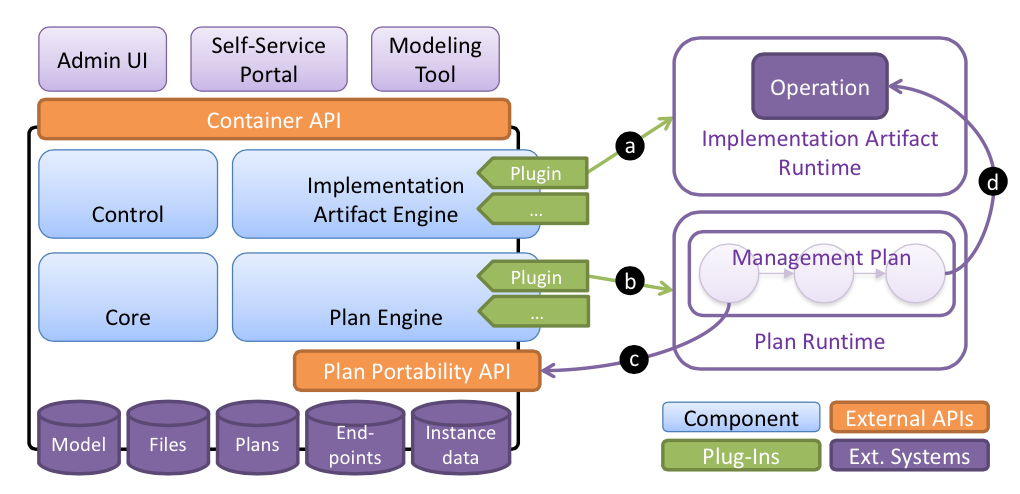
\includegraphics[width=\textwidth]{images/open_container}
  \caption{OpenTOSCA Architecture Overview and Processing Sequence.}
  \label{fig:open_container}
\end{figure}\\
Requests to the Container API are redirected to the Control module, that is responsible to orchestrate the different components, track their progress and interprets the TOSCA application.
The Core module provides common services to other components, e. g., managing data or validating XML. The Implementation Artifact Engine is responsible to run the Implementation Artifact
contained in the CSAR in order to make them available for plans, usually these Implementation Artifacts provides management operations of nodes and relationships. The Plan Engine is responsible
to process the management plans contained in CSARs, they also employs plugins to support different workflow languages, usually BPMN or BPEL, and their runtime environments. The portability of
management plans between different environments and runtimes is ensured by the Plan Portability API. Plans only provides an abstract description of the required service, it is responsibility of
the plan plugin to bind the services invoked by the plans to the endpoint of the management operation before it deploys the plan to the respective workflow runtime.
% --------------------------------------------
% WINERY
% --------------------------------------------
\subsubsection{Winery}
\label{subs:Winery}
Winery is web-based tool that enable modeling of TOSCA-based applications and creation CSARs in a tailored environment \cite{Winery}. Its main features are type management and graphical topology modeling where the defined types
are instantiated and interlinked. Winery architecture is composed essentially of three parts, the Topology Modeller, the Element Manager, and the Repository, where all data is stored, as illustrated in Figure~\ref{fig:winery}.
% --------------------------------------------
% WINERY ARCHITECTURE
% --------------------------------------------
\begin{figure}[h!]
  \centering
  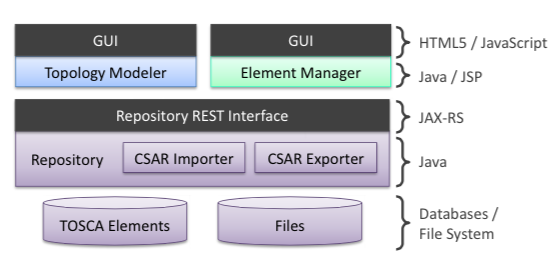
\includegraphics[width=\textwidth]{images/winery}
  \caption{Winery Architecture.}
  \label{fig:winery}
\end{figure}\\
The Topology Modeller makes modeling of application easier by depicting element and combinations thereof visually, that allows to architects, developers and operators to understand the and model applications without the need for
technical knowledge of type implementations and configurations, that is possible because the Topology Modeller handle only with the TOSCA meta models that are directly related to visual topology modeling, such as the node templates,
relationship templates, deployment artifacts, requirements and policy. In the other hand the meta models that are used to define semantics and configurations such as types, implementations and policy templates are only created, modified
and deleted exclusively by the Element Manager. By accessing the Element Manager, technical experts to provide and configure node types and relationships.
% --------------------------------------------
% VINOTHEK
% --------------------------------------------
\subsubsection{Vinothek}
\label{subs:Vinothek}
Vinothek \cite{breitenbucher2014vinothek} is a web-based Self-Service portal that allows end-users to provision new TOSCA-based application instances through a simple graphical interface, as illustrated in Figure~\ref{fig:vinothek}.
\begin{figure}[h!]
  \centering
  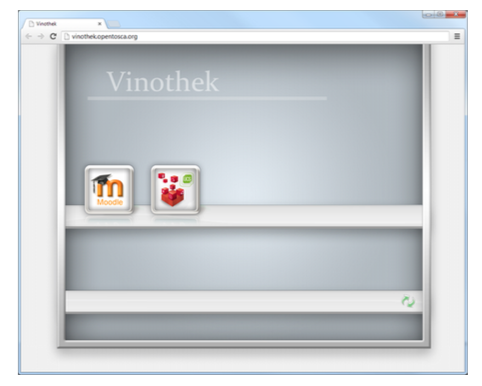
\includegraphics[width=.5\textwidth]{images/vinothek}
  \caption{Vinothek Self-Service Portal}
  \label{fig:vinothek}
\end{figure}\\
Vinothek abstracts the technical details and differences of different TOSCA Runtimes and provides a single interface to provision the applications. To perform the provision of the applications, Vinothek communicates with the server that
delegates calls to the \textit{TOSCA Application Lifecycle Manager} via a \textit{RESTFUL API}, as illustrated on Figure~\ref{fig:vinothek_architecture}.
\begin{figure}[h!]
  \centering
  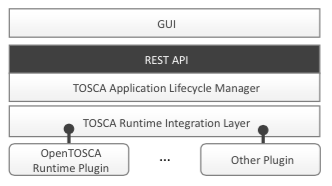
\includegraphics[width=.5\textwidth]{images/vinothek_architecture}
  \caption{Vinothek Self-Service Portal Architecture}
  \label{fig:vinothek_architecture}
\end{figure}\\
Currently the \textit{Application Lifecycle Manager} only supports dealing with the provisioning of applications, in the future it will support dealing with management and termination of applications. Another component of Vinothek is the
\textit{TOSCA Runtime Integration Layer} that is responsible to provide the mechanisms to plug-in TOSCA Runtimes. Although Vinothek facilitates the provisioning of applications, there are key mechanisms identified by the authors that currently Vinothek
does not provide and are important in the application lifecycle such as performing management functionalities and processing policies to define security and other non-functional requirements.
% --------------------------------------------
% FOSSTRAK EPCIS
% --------------------------------------------
\subsection{Fosstrak EPCIS}
\label{sub:Fosstrak EPCIS}
This sections will describe what is the Fosstrak EPCIS framework. How this framework is relationed with IoT applications?
